\documentclass[a4paper, 12pt, finnish]{report}
\usepackage[utf8]{inputenc}
\usepackage{amsfonts}
\usepackage{graphics}
\usepackage[finnish]{babel}
\usepackage{titlesec}
\titleformat{\chapter}
{\Large\bfseries}
{}            
{0pt}      
{\huge} 

\newcommand{\topic}{Hakemukseni AYYn hallitukseen kaudelle 2017}
\usepackage{hyperref}
\hypersetup{pdfpagemode=UseNone, pdfstartview=FitH, colorlinks=true,urlcolor=red,linkcolor=blue,citecolor=black,pdftitle={\topic},pdfauthor={Onni Lampi}}
\setlength{\parindent}{0mm}
\setlength{\emergencystretch}{15pt}
\newcommand*{\findate}{\the\day.\the\month.\the\year}

\begin{document}



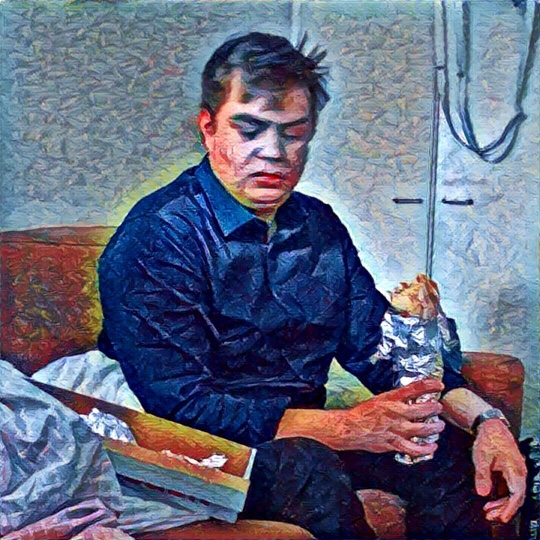
\includegraphics{Onni.jpg}
\section*{\topic}

Olen 24-vuotias 4. vuoden tietoliikennetekniikan opiskelija.
Olen kotoisin Helsingistä ja tässä muutaman opiskeluvuoden aikana AYY on tullut minulle hyvin läheiseksi ja rakkaaksi organisaatioksi.
Siksi haenkin AYYn hallitukseen, jotta pääsen ylioppilaskunnan organisaation sydämeen vaikuttamaan ja toteuttamaan konkreettisia asioita.\\

Olen pitkään miettinyt hallitukseen hakemista, mutta empinyt niin suuren tehtävän edessä.
Aloin kuitenkin puhua asiasta varovaisesti syksyn aikana ja kaikki asiasta kuulleet ihmiset innostuivat ideasta heti.
Ihmiset ihmettelivät, miksen ollut hakenut hallitukseen jo aiemmin tai miksi en pidä asiasta suurempaa ääntä.
Tämä vakuutti minut siitä, että olisin hallitukseen sopiva ylioppilaskunnan ja sen jäsenet tunteva henkilö.\\

Olen toiminut erinäisissä vapaaehtoishommissa ylioppilaskunnassa käytännössä koko opiskeluaikani.
Näihin kuuluu mm. vastuut edustajistossa toimimisesta Radiodiodin päätoimittajana toimimiseen.
Täydellinen lista vastuutehtävistä ja muista nakeistani löytyy ohessa olevasta CV:stäni. :)\\

Persoonana olen rauhallinen, tunnollinen ja huumorintajuinen.
Vastuuni hoidan jämäkästi ja harkiten, en hätiköi asioita turhaan.
Pikaista reagointia vaativissa tilanteissa olen kyllä hyvä tekemään nopeita päätöksiä ja tässä auttaa aiemmin hankittu kokemus.
Rehellisesti sanottuna edellä mainitut tilanteet eivät ole suurinta mukavuusaluettani, mutta niistäkin olen aina selvinnyt kunnialla.\\

Olen hyvä toimimaan osana tiimiä ja tuon porukkaan mukavaa letkeyttä.
En kuitenkaan pidä turhasta tauhkasta hommia tehdessä (varsinkaan kokoustaessa) vaan mielelläni hoidan kokouksissa ja tapaamisissa ensin asiat alta pois, tämän jälkeen sitten huvit!\\

Hallituksessa minua erityisesti kiinnostaa kiinteistöt ja viestintä.
Kiinteistöt ovat hyvin konkreettinen osa-alue AYYn tarjoamissa palveluissa ja olisin loistava henkilö vetämään niille ensi vuoden toimintasuunnitelmassa kuvattuja projekteja.
Tietotaitoni viestinnän ja erinäisten teknologioiden suhteen olisi hyödyksi kiinteistöpalvelujen digitalisaatiossa.
Ylioppilaskunnan viestintä yleensäkin kiinnostaa minua suuresti ja sekin on minua mielyttävä hyvin konkreettinen osa-alue.\\

Terveisin, Onni

Espoossa \findate

\subsection*{Kysykää ihmeessä lisää!}
Onni Lampi\\
040 702 3841\\
omnez@IRCnet, telegram\\
contact@onnilampi.fi

\end{document}
